% Provenance (never printed): see sources/outline_sources.md (Year 2: Hadean, Archean and
% Proterozoic; early crust and greenstone belts; the oxygenation of the atmosphere; snowball
% Earth). Eons and eras from the ICS chart; greenstone belts, TTG and cratons after Cawood and
% others (2018) and Smithies and others (2019); komatiite liquidus after Sossi and O'Neill (2016),
% Pierru and others (2022) and Asimow (2022); the Archean air and the GOE after Catling and Zahnle
% (2020) and Luo and others (2016); the boring billion after Lyons and others (2021); snowball
% Earth after Hoffman and others (2017). The energy-balance model, the komatiite line and the CO2
% build-up from figdata/bachelor-2/precambrian.py; exercise and problem values in the Book 4
% scratch calculator calc/ch18.py.
\chapter{De precambrische Aarde}\label{ch:b2:precambrian-earth}

De eerste schelpdragende fossielen verschijnen in gesteenten van ongeveer 540 miljoen jaar oud. Alles daarvoor, vanaf
de geboorte van de Aarde \qty{4567}{Ma} geleden, is het Precambrium: zeven achtste van de geschiedenis
van de planeet. In die tijd bouwde de Aarde de kernen van haar continenten, vulde ze haar lucht met zuurstof,
en bevroor ze minstens twee keer van de polen tot de evenaar, met ijskappen die in de tropen
de zee bereikten. Dit hoofdstuk leest die vier miljard jaar af aan de gesteenten die eruit zijn overgebleven,
en drukt drie van hun raadsels in getallen uit: waarom de oudste lava's zo heet waren, hoe een bevroren
planeet kan ontdooien, en hoe de jonge Aarde warm bleef onder een zwakke Zon.
% ledger: ics:base.Hadean, ics:base.Phanerozoic, hoffman17:cryochrons

\begin{recall}
\textbf{Uit de schoolboeken}: de ouderdom van de Aarde; de eonen op de geologische tijdschaal;
de wet voor de lichtkracht van de jonge Zon en het \omterm{def:b2:precambrian-earth:faint-sun}{probleem van de zwakke jonge Zon}; de oeratmosfeer;
stromatolieten, \omterm{def:b2:precambrian-earth:bif}{gebande ijzerformaties}, de \omterm{def:b2:precambrian-earth:goe}{Grote Oxidatie} en rode lagen; \omterm{def:b2:precambrian-earth:craton}{cratons};
radiogene warmte in het verleden. \textbf{Uit Boek~3}: zirkoon en zijn U--Pb-ouderdommen,
sluitingstemperatuur; de radiogene warmteproductie van de vier isotopen; uitgaande langgolvige
straling en de wereldgemiddelde instraling $S_0/4$; chronostratigrafische eenheden.
\textbf{Uit eerdere hoofdstukken}: de potentiële temperatuur van de mantel en de adiabaat
(\cref{ch:b2:mantle-melting}); de liquidus en de \omterm{def:b2:magmatic-differentiation:crystallisation}{fractionele kristallisatie} van olivijn
(\cref{ch:b2:magmatic-differentiation}); de graniettypes (\cref{ch:b2:crustal-melting});
\omterm{def:b2:wilson-cycle:supercontinent}{supercontinenten} (\cref{ch:b2:wilson-cycle}). Oxidatie en reductie horen bij de
scheikundeboeken, en de eerste eukaryoten en de fotosynthese bij de biologieboeken.
\end{recall}

\section{Drie eonen vóór de fossielen}\label{sec:b2:precambrian-earth:eons}

\begin{definition}[Hadeïcum, Archaïcum, Proterozoïcum]\label{def:b2:precambrian-earth:eons}
De tijd vóór het Fanerozoïcum wordt in drie eonen verdeeld. Het \emph{Hadeïcum}\index{Hadeïcum}
loopt van de vorming van de Aarde, \qty{4567}{Ma} geleden, tot $4031 \pm \qty{3}{Ma}$; het
\emph{Archaïcum}\index{Archaïcum} van $4031$ tot \qty{2500}{Ma}; het
\emph{Proterozoïcum}\index{Proterozoïcum} van 2500 tot \qty{538.8}{Ma}, de basis van het Cambrium.
Samen worden ze informeel het Precambrium genoemd.
\end{definition}
% ledger: ics:base.Hadean, ics:base.Archean, ics:base.Proterozoic, ics:base.Phanerozoic

Het \omterm{def:b2:precambrian-earth:eons}{Archaïcum} wordt in vier era's verdeeld, het Eoarchaïcum (4031 tot \qty{3600}{Ma}), Paleoarchaïcum (3600
tot 3200), Mesoarchaïcum (3200 tot 2800) en Neoarchaïcum (2800 tot 2500); het \omterm{def:b2:precambrian-earth:eons}{Proterozoïcum} in drie,
het Paleoproterozoïcum (2500 tot \qty{1600}{Ma}), Mesoproterozoïcum (1600 tot 1000) en
Neoproterozoïcum (1000 tot 538.8). Twee neoproterozoïsche perioden zijn hieronder van belang, het Cryogenium, 720 tot
\qty{635}{Ma}, en het Ediacarium, 635 tot \qty{538.8}{Ma}.
% ledger: ics4:archean-eras, ics4:proterozoic-eras

\begin{omfigure}
\centering
% ledger: ics:base.Hadean, ics:base.Archean, ics:base.Proterozoic, ics:base.Phanerozoic, ics4:archean-eras, ics4:proterozoic-eras, wilde01:4404, bowring99:acasta, cz20:impacts, allwood06:spc, cawood18:transition, gumsley17:goe, luo16:goe, hoffman17:earlier, earle:bif, lyons21:boring, hoffman17:ages, asimow22:komatiite
\begin{tikzpicture}[x=-3.4cm, y=1cm, font=\scriptsize]
% eons
\fill[icsHadean] (4.567,0) rectangle (4.031,0.5);
\fill[icsArchean] (4.031,0) rectangle (2.5,0.5);
\fill[icsProterozoic] (2.5,0) rectangle (0.5388,0.5);
\fill[icsPhanerozoic] (0.5388,0) rectangle (0,0.5);
\node[text=white] at (4.299,0.25) {Hadeïcum};
\node[text=white] at (3.27,0.25) {Archaïcum};
\node[text=white] at (1.52,0.25) {Proterozoïcum};
\node at (0.27,0.25) {Fan.};
% eras
\foreach \a/\b/\c in {4.031/3.6/35, 3.6/3.2/55, 3.2/2.8/35, 2.8/2.5/55}
  \fill[icsArchean!\c] (\a,-0.45) rectangle (\b,0);
\foreach \a/\b/\c in {2.5/1.6/35, 1.6/1.0/55, 1.0/0.5388/35}
  \fill[icsProterozoic!\c] (\a,-0.45) rectangle (\b,0);
\foreach \x/\l in {3.8155/Eo, 3.4/Paleo, 3.0/Meso, 2.65/Neo, 2.05/Paleo, 1.3/Meso, 0.769/Neo}
  \node at (\x,-0.225) {\l};
% axis
\draw (4.6,-0.6) -- (0,-0.6);
\foreach \t in {0,0.5,...,4.5} {
  \draw (\t,-0.6) -- (\t,-0.7);
  \node[anchor=north] at (\t,-0.7) {\pgfmathprintnumber[fixed, precision=1]{\t}};
}
\node[anchor=north, font=\small] at (2.3,-1.05) {tijd vóór heden (miljard jaar)};
% row A
\fill[omDef] (4.404,0.85) circle (2pt);
\node[anchor=west, text=omDef] at (4.404,0.85) {oudste zirkoon};
\fill[omMeth] (3.43,0.85) circle (2pt);
\node[anchor=west, text=omMeth] at (3.43,0.85) {eerste stromatolieten};
\draw[red!60!black, line width=3pt] (2.4,0.85) -- (1.8,0.85);
\node[anchor=west, text=red!60!black] at (1.8,0.85) {gebande ijzerformaties};
% row B
\fill[omDef] (4.03,1.5) circle (2pt);
\node[anchor=west, text=omDef] at (4.03,1.5) {oudste gesteenten};
\draw[black!70, line width=3pt] (3.2,1.5) -- (2.5,1.5);
\node[anchor=south, text=black!80] at (2.85,1.6) {verandering van tektonische stijl};
\draw[omProp, line width=3pt] (1.8,1.5) -- (0.8,1.5);
\node[anchor=south, text=omProp] at (1.3,1.6) {``saai miljard''};
% row C
\draw[black!60, line width=2pt, densely dashed] (4.2,2.25) -- (3.5,2.25);
\node[anchor=south, text=black!70] at (3.85,2.35) {laat zwaar bombardement? (omstreden)};
\draw[omThm, line width=3pt] (2.43,2.25) -- (2.06,2.25);
\node[anchor=west, text=omThm] at (2.06,2.25) {Grote Oxidatie};
% row D
\fill[blue!60!black] (2.4,3.0) circle (2pt);
\node[anchor=east, text=blue!60!black] at (2.4,3.0) {eerste sneeuwbalaarde};
\fill[omThm] (0.8,3.0) circle (2pt);
\node[anchor=east, text=omThm] at (0.8,3.0) {tweede zuurstofstijging};
% row E
\fill[orange!80!black] (1.9,3.7) circle (2pt);
\node[anchor=east, text=orange!80!black] at (1.9,3.7) {laatste gewone komatiieten};
\draw[blue!60!black, line width=3pt] (0.717,3.7) -- (0.635,3.7);
\node[anchor=east, text=blue!60!black] at (0.717,3.7) {cryogene sneeuwbalaardes};
% row F
\fill[omMeth] (0.57,4.4) circle (2pt);
\node[anchor=east, text=omMeth] at (0.57,4.4) {eerste grote fossielen (Ediacarium)};
\end{tikzpicture}
\par\smallskip{\small Het Precambrium op één lijn. De eonen en, in lichtere tinten, hun era's
(Eo-, Paleo-, Meso- en Neoarchaïcum; Paleo-, Meso- en Neoproterozoïcum) zijn die van de
Internationale Chronostratigrafische Kaart; de gebeurtenissen staan bij de ouderdommen die in de tekst worden genoemd.
De ``laatste gewone \omterm{def:b2:precambrian-earth:greenstone}{komatiieten}'' zijn die zonder aluminiumverarming; jongere, zeldzamere soorten bestaan.}
\end{omfigure}

\subsection*{Het Hadeïcum: mineralen zonder gesteenten}

Uit het \omterm{def:b2:precambrian-earth:eons}{Hadeïcum} is geen gesteente overgebleven, alleen mineralen. Het oudste is een zirkoonkorrel uit de Jack
Hills in West-Australië, $4404 \pm \qty{8}{Myr}$ oud, uit een ouder gesteente gespoeld en
ongeveer drie miljard jaar geleden in een conglomeraat afgezet. Zijn samenstelling, en die van zijn
buren, werd door zijn ontdekkers gelezen als bewijs dat een korst van continentaal type en
vloeibaar water al \qty{4.4}{Gyr} geleden bestonden, zo'n 160 miljoen jaar nadat de Aarde
ontstond. De oudste gedateerde gesteenten, de Acasta-gneisen in het noordwesten van Canada, zijn 4.00 tot
\qty{4.03}{Ga} oud, dicht bij de basis van het \omterm{def:b2:precambrian-earth:eons}{Archaïcum}.
% ledger: wilde01:4404, wilde01:zircon, uw14:jack-hills, bowring99:acasta

De jonge Aarde werd getroffen door grote hemellichamen, zoals \cref{ch:b2:planet-formation-meteorites}
beschreef. De laatste inslag die groot genoeg was om
de hele oceaan te verdampen, vond naar schatting ongeveer \qty{4.3}{Ga} geleden plaats. Een later ``laat zwaar
bombardement'', een uitbarsting van inslagen tussen ongeveer 4.2--4.0 en \qty{3.5}{Ga}, afgeleid uit de
ouderdommen van maangesteenten en van schokken in \omterm{def:b2:planet-formation-meteorites:fall-find}{meteorieten}, is voorgesteld; velen betwisten dat het überhaupt een
afzonderlijke gebeurtenis was, en hoe dan ook zou het de Aarde waarschijnlijk niet hebben gesteriliseerd.
% ledger: cz20:impacts

\section{De archaïsche korst}\label{sec:b2:precambrian-earth:archean}

\subsection*{Groensteengordels en komatiieten}

De archaïsche korst die is overgebleven, bestaat uit twee soorten terrein, naast elkaar: grote lichamen van
grijze, natriumrijke granitische gneis, en smallere gordels van omgezet vulkanisch en sedimentair gesteente.

\begin{definition}[Groensteengordel; komatiiet]\label{def:b2:precambrian-earth:greenstone}
Een \emph{groensteengordel}\index{groensteengordel} is een gordel van mafische en ultramafische vulkanische gesteenten,
met sedimenten, laaggradig gemetamorfoseerd (het groen komt van chloriet, actinoliet en
epidoot), die tussen granitoïde lichamen ligt in archaïsche en sommige proterozoïsche terreinen. Een
\emph{komatiiet}\index{komatiiet} is een ultramafische lava, veel rijker aan MgO dan basalt,
die als vloeistof werd uitgestoten; zijn olivijn groeit typisch in lange, dunne bladen, de
\emph{spinifextextuur}, terwijl de top van de stroom snel afkoelt.
\end{definition}
% ledger: cawood18:dome-keel, so16:liquidus, pierru22:komatiite

\begin{omfigure}
\centering
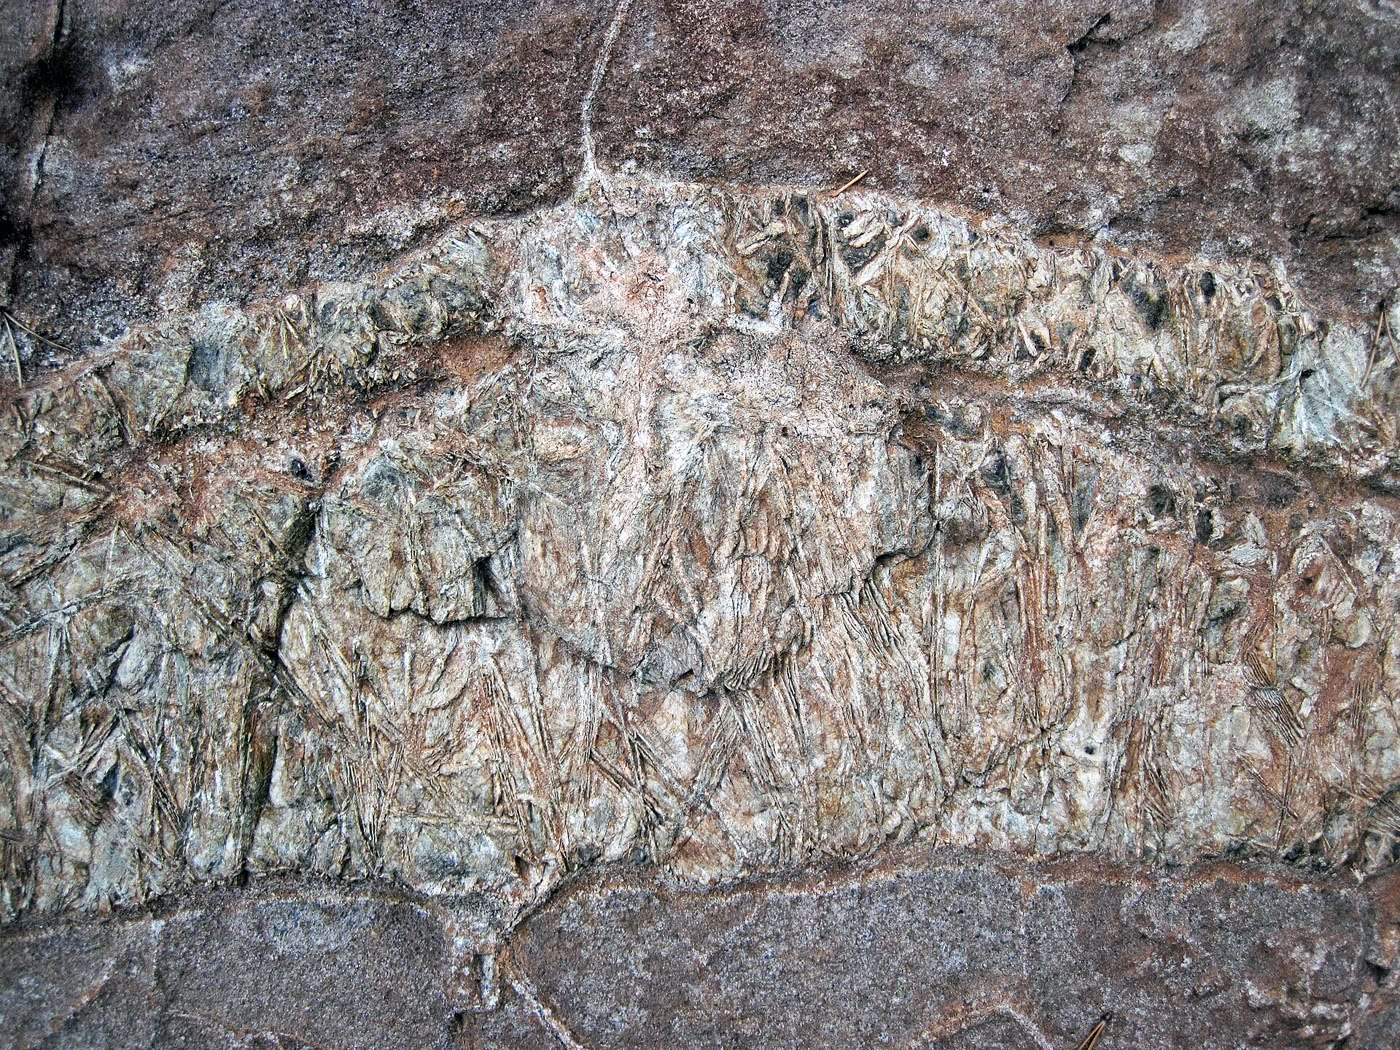
\includegraphics[width=0.66\linewidth]{images/book4/b2-18-spinifex-komatiite.jpg}
\par\smallskip{\small Spinifextextuur in een komatiietstroom, Pyke Hill, Ontario, deel van een
neoarchaïsche \omterm{def:b2:precambrian-earth:greenstone}{groensteengordel} van ongeveer 2.71 miljard jaar oud: bladen van olivijn, nu omgezet,
groeiden dwars door de afkoelende top van de stroom. Foto James St.~John, CC~BY~2.0 (Wikimedia
Commons).}
\end{omfigure}

\omterm{def:b2:precambrian-earth:greenstone}{Komatiieten} bevatten tot \qty{34}{\percent} MgO, tegen 10 tot \qty{13}{\percent} in de primaire
basalten van de huidige ruggen, en ze zijn bijna beperkt tot de oude Aarde: de soort met aluminiumverarming
komt alleen voor in gesteenten ouder dan \qty{2.8}{Ga}, de soort zonder aluminiumverarming tot ongeveer
\qty{1.9}{Ga}, en alleen een zeldzame, met aluminium verrijkte soort is zo jong als \qty{90}{Myr}. Een smelt
die zo rijk aan magnesium is, is zeer heet, en, zoals voor de basalten van
\cref{ch:b2:magmatic-differentiation}, is olivijn het eerste mineraal dat eruit kristalliseert;
het aandeel ervan in de vloeistof legt de temperatuur vast.
% ledger: pierru22:komatiite, asimow22:komatiite

\begin{proposition}[De komatiietthermometer]\label{prop:b2:precambrian-earth:liquidus}
Voor een smelt in evenwicht met olivijn bij atmosferische druk stijgt de liquidustemperatuur
bijna lineair met het MgO-gehalte van de smelt. Door twee experimenten $(m_1, T_1)$ en
$(m_2, T_2)$ geldt
\[
  T_{\text{liq}}(m) = T_1 + s\,(m - m_1), \qquad s = \frac{T_1 - T_2}{m_1 - m_2} .
\]
Smeltexperimenten op twee \omterm{def:b2:precambrian-earth:greenstone}{komatiieten}, $\qty{32.2}{\percent}$ MgO bij \qty{1616}{\celsius} en
$\qty{23}{\percent}$ bij \qty{1450}{\celsius}, geven $s = \qty{18.0}{\celsius}$ per procent
MgO.
\end{proposition}
% ledger: so16:liquidus, helz98:glass-thermometer

\begin{proof}
Olivijn is een vaste oplossing van forsteriet en fayaliet, veel rijker aan magnesium dan de smelt
waaruit het groeit. Terwijl de smelt afkoelt, onttrekt olivijn er magnesium aan, en de temperatuur
waarbij de smelt net verzadigd is aan olivijn daalt met zijn MgO-gehalte. Experimenten tonen dat
de daling over het bereik van een gegeven familie van smelten bijna lineair is, zodat de lijn door
twee experimenten ertussen interpoleert; $s = (1616 - 1450)/(32.2 - 23) = 166/9.2 = 18.04$.
\end{proof}

De coëfficiënt is niet eigen aan \omterm{def:b2:precambrian-earth:greenstone}{komatiieten}. Glazen die uit de lava van de Kilauea zijn afgeschrikt,
op dezelfde manier geijkt, veranderen met \qty{3}{\celsius} voor \qty{0.15}{\percent} MgO, dat
is \qty{20}{\celsius} per procent. Door de komatiietlijn door te trekken tot een primair rugbasalt
met \qty{12}{\percent} MgO vindt men dus zijn liquidus tot op enkele tientallen graden: $1616 -
18.0\times20.2 \approx \qty{1252}{\celsius}$. De heetste komatiietvloeistoffen waren dus
zo'n \qty{360}{\celsius} heter dan de smelten die de huidige ruggen voeden, en de figuur hieronder
toont de lijn.
% ledger: helz98:glass-thermometer, so16:liquidus, pierru22:komatiite
% values: slope 18.043, T_morb12 1251.5, dT_kom_morb 364.5 (precambrian.py)

\begin{omfigure}
\centering
\begin{tikzpicture}
\begin{axis}[omrecord, width=0.72\linewidth, height=6cm, xmin=8, xmax=35, ymin=1150, ymax=1700,
  xlabel={MgO in de smelt (\unit{\percent} in massa)}, ylabel={liquidus bij 1 atm (\unit{\celsius})},
  xtick pos=bottom, ytick pos=left, clip=false,
  y tick label style={/pgf/number format/1000 sep={}}]
% computed in figdata/bachelor-2/precambrian.py part kom; ledger: so16:liquidus, pierru22:komatiite
\fill[omProp!15] (axis cs:10,1150) rectangle (axis cs:13,1700);
\addplot[black, line width=1.1pt] table[x=MgO, y=T] {figdata/out/bachelor-2-precambrian-kom.dat};
\addplot[only marks, mark=*, mark size=2.4pt, omThm] coordinates {(32.2,1616) (23,1450)};
\node[anchor=north west, font=\scriptsize, text=omThm] at (axis cs:32.2,1612) {Barberton};
\node[anchor=north west, font=\scriptsize, text=omThm] at (axis cs:23,1446) {Munro};
\node[anchor=south, font=\scriptsize, text=omProp, align=center] at (axis cs:11.5,1560)
  {primaire\\rugbasalten};
\draw[densely dashed] (axis cs:12,1150) -- (axis cs:12,1251.5) -- (axis cs:8,1251.5);
\draw[densely dashed] (axis cs:32.2,1150) -- (axis cs:32.2,1616);
\draw[<->, omDef, thick] (axis cs:27,1251.5) -- (axis cs:27,1616);
\draw[densely dotted] (axis cs:12,1251.5) -- (axis cs:27,1251.5);
\draw[densely dotted] (axis cs:27,1616) -- (axis cs:32.2,1616);
\node[anchor=east, font=\scriptsize, text=omDef] at (axis cs:26.7,1330) {ongeveer \qty{360}{\celsius}};
\end{axis}
\end{tikzpicture}
\par\smallskip{\small De komatiietthermometer: de lijn door de liquidustemperaturen
gemeten op twee \omterm{def:b2:precambrian-earth:greenstone}{komatiieten} (stippen), doorgetrokken tot de 10 tot \qty{13}{\percent} MgO van de primaire
basalten van de huidige ruggen (band). De verlenging berust op de vergelijkbare helling van basaltische smelten.}
\end{omfigure}

Hetere lava betekent niet een mantel die evenveel heter is. \omterm{def:b2:precambrian-earth:greenstone}{Komatiieten} stegen waarschijnlijk op in
pluimen, zoals de heetste basalten vandaag op Hawaï doen, waar de potentiële temperatuur tot
ongeveer \qty{200}{\celsius} boven de $1350 \pm \qty{50}{\celsius}$ van de omringende mantel ligt. En
ze ontstonden door hoge smeltgraden, op grotere diepte. Algemeen wordt aangenomen dat ze zich
vormden in een mantel die 200 tot \qty{300}{K} warmer was dan vandaag; een alternatieve opvatting stelt dat
\omterm{def:b2:precambrian-earth:greenstone}{komatiieten} natte \omterm{def:b2:magma-emplacement:magma}{magma's} waren, gevormd bij temperaturen die niet veel hoger lagen dan die van de omringende
mantel. Hoe dan ook was de archaïsche mantel heter, en de schoolboeken
gaven één reden: 3 miljard jaar geleden gaven de vier radioactieve isotopen meer dan
twee keer de huidige warmte af (\cref{exo:b2:precambrian-earth:2}).
% ledger: asimow22:komatiite, pierru22:komatiite, so16:liquidus

\subsection*{TTG en het koepel-en-kielpatroon}

De grijze gneisen tussen de \omterm{def:b2:precambrian-earth:greenstone}{groensteengordels} zijn geen granieten van het soort dat
\cref{ch:b2:crustal-melting} beschreef.

\begin{definition}[Tonaliet--trondhjemiet--granodiorietreeks]\label{def:b2:precambrian-earth:ttg}
De \emph{tonaliet--trondhjemiet--granodiorietreeks}\index{tonaliet--trondhjemiet--granodiorietreeks}
(TTG) is de familie van natriumrijke, kaliumarme granitoïden --- tonalieten,
trondhjemieten (tonalieten arm aan mafische mineralen) en granodiorieten --- die het grootste deel van
de archaïsche continentale korst vormt. De meeste ontstonden door \omterm{def:b2:mantle-melting:melting}{partieel smelten} van gehydrateerde basaltische
korst.
\end{definition}
% ledger: smithies19:ttg, cawood18:ttg

Een groot deel van het volume van de huidige continentale korst was aan het einde van het \omterm{def:b2:precambrian-earth:eons}{Archaïcum} gevormd, grotendeels
als TTG. Sommige TTG dragen sporenelementsignaturen die lang werden gelezen als smelten op meer dan
\qty{50}{km} diepte, een druk die in jongere continentale korst niet wordt bereikt, en die lezingen
wegen mee in het debat over wanneer de platentektoniek begon; een studie uit 2019 betoogde dat die signaturen
in plaats daarvan van smelten uit de mantel komen, en dat de gewone TTG zich vormde op
diepten van niet meer dan de \qty{40}{km} van een gewone continentale korst vandaag. Laat in het
\omterm{def:b2:precambrian-earth:eons}{Archaïcum}, tussen ongeveer 3.0 en \qty{2.5}{Ga}, gaan de granitoïden van de meeste \omterm{def:b2:precambrian-earth:craton}{cratons} over van TTG
naar kaliumrijke granieten, het teken dat een dikkere korst opnieuw werd gesmolten.
% ledger: smithies19:ttg, cawood18:ttg

In het oosten van de Pilbara in Australië, in Zimbabwe en in het zuiden van India tekenen de twee terreinen een
opvallend patroon op de kaart. Ronde koepels van granitoïde worden omlijst door synclinale kielen van groensteen waarvan de lagen van de koepels af hellen en ook van de koepels af jonger worden. Men
denkt dat de koepels als \omterm{def:b2:magma-emplacement:ascent}{diapieren} zijn opgestegen: lichte granitische korst die opsteeg door een dikke, dichte stapel
lava's die ertussen wegzonk. In de Pilbara ging deze koepelvorming honderden miljoenen
jaren door en stopte ze ongeveer \qty{3.1}{Ga} geleden, waarna de structuren lineair worden, zoals die
van jongere \omterm{def:b2:alpine-orogen:orogen}{orogenen}.
% ledger: cawood18:dome-keel

\begin{omfigure}
\centering
\begin{tikzpicture}[x=0.95cm, y=0.95cm, font=\scriptsize]
% schematic, after the description in cawood18:dome-keel
\fill[lith basalt] (0,0) rectangle (12,7);
\draw (0,0) rectangle (12,7);
\foreach \cx/\cy/\rx/\ry in {2.4/4.7/1.7/1.4, 7.2/5.0/2.0/1.4, 4.6/1.6/1.9/1.1, 10.0/2.0/1.4/1.3}
  \filldraw[lith granite, draw=black, thick] (\cx,\cy) ellipse ({\rx} and {\ry});
% strekking en helling in de groensteen, elk van de dichtstbijzijnde koepel af hellend
% (positions and strikes from the outward normals of the ellipses, computed by hand)
\foreach \px/\py/\st in {3.9/5.99/309, 0.9/5.99/231, 0.9/3.41/129, 2.4/2.88/90, 4.52/4.7/0,
    9.62/5.0/0, 8.91/6.29/305, 5.49/6.29/235, 8.91/3.71/55, 5.49/3.71/125,
    6.92/1.6/0, 4.6/3.12/270, 2.28/1.6/180, 6.24/0.53/60,
    10.0/3.72/270, 11.29/0.78/47, 8.18/2.0/180, 11.29/3.22/313}
  \pic at (\px,\py) {strikedip={\st}{}};
\node[fill=white, inner sep=1.5pt] at (2.4,4.7) {TTG-koepel};
\node[fill=white, inner sep=1.5pt] at (7.2,5.0) {TTG-koepel};
\node[fill=white, inner sep=1.5pt] at (4.6,1.6) {TTG-koepel};
\node[fill=white, inner sep=1.5pt] at (10.0,2.0) {TTG-koepel};
\node[fill=white, inner sep=1.5pt, align=center] at (7.45,2.75) {groensteen-\\kiel};
\node[fill=white, inner sep=1.5pt, align=center] at (1.0,0.9) {groensteen};
\pic at (11.4,5.6) {northarrow};
% section below
\begin{scope}[yshift=-3.3cm]
\fill[lith basalt] (0,0) -- (12,0) -- (12,2.2) -- (0,2.2) -- cycle;
\filldraw[lith granite, draw=black, thick] (0.6,0) .. controls (0.6,2.0) and (4.6,2.0) .. (4.6,0) -- cycle;
\filldraw[lith granite, draw=black, thick] (6.4,0) .. controls (6.4,2.1) and (11.0,2.1) .. (11.0,0) -- cycle;
\draw[thick] (0,0) rectangle (12,2.2);
\draw[black!70] (4.6,0.9) .. controls (5.5,0.2) .. (6.4,0.9);
\draw[black!70] (4.35,1.5) .. controls (5.5,0.6) .. (6.65,1.5);
\node[fill=white, inner sep=1.5pt] at (2.6,0.6) {TTG};
\node[fill=white, inner sep=1.5pt] at (8.7,0.6) {TTG};
\node[fill=white, inner sep=1.5pt] at (5.5,1.75) {kiel};
\draw[->, thick] (2.6,1.0) -- (2.6,1.75);
\draw[->, thick] (8.7,1.05) -- (8.7,1.8);
\draw[->, thick] (5.5,1.4) -- (5.5,0.95);
\node[anchor=west] at (12.1,1.1) {doorsnede};
\end{scope}
\node[anchor=west] at (12.1,3.5) {kaart};
\end{tikzpicture}
\par\smallskip{\small Het koepel-en-kielpatroon van sommige archaïsche \omterm{def:b2:precambrian-earth:craton}{cratons} (schematisch, niet op
schaal). Kaart: granitoïde koepels van de TTG-reeks omlijst door groensteen; de
strekking-en-hellingssymbolen tonen dat de lagen van de groenstenen van elke koepel af hellen. Doorsnede: de koepels
rijzen terwijl de dichte groensteenstapel ertussen in synclinale kielen wegzinkt (pijlen).}
\end{omfigure}

\subsection*{Cratons}

\begin{definition}[Craton]\label{def:b2:precambrian-earth:craton}
Een \emph{craton}\index{craton} is een deel van een continent dat meer dan een miljard jaar tektonisch stabiel
is gebleven: een kern van archaïsche of proterozoïsche korst, metamorf en
plutonisch, die rust op een dikke, koude en drijvende wortel van lithosferische mantel die tot zo'n
\qty{250}{km} diep reikt.
\end{definition}
% ledger: tulane:cratons, fischer:lithosphere, cawood18:ttg

De \omterm{def:b2:precambrian-earth:craton}{cratons} stabiliseerden grotendeels in het Mesoarchaïcum en Neoarchaïcum, en de tekenen van hun
stabiliteit staan in de gesteenten geschreven: brede sedimentaire bekkens die erop werden afgezet, zoals de
Transvaal-supergroep op het Kaapvaalcraton (ongeveer 2640 tot \qty{2055}{Ma}) en de Mount Bruce-supergroep
op de Pilbara (2775 tot \qty{2210}{Ma}); zwermen van rechte \omterm{def:b2:magma-emplacement:bodies}{gangen} die ze doorsnijden als
brosse platen; en hun dikke wortels, verworven tegen het late \omterm{def:b2:precambrian-earth:eons}{Archaïcum}. Tussen 3.2 en
\qty{2.5}{Ga} toont het archief ook de oudste passieve randen en \omterm{def:b2:alpine-orogen:foreland}{voorlandbekkens}, gordels
van gepaarde \omterm{def:b2:metamorphic-facies:metamorphism}{metamorfose}, en paleomagnetisch bewijs dat \omterm{def:b2:precambrian-earth:craton}{cratons} ten opzichte van elkaar bewogen.
Een overzichtsartikel uit 2018 leest deze veranderingen als het geleidelijke begin van de platentektoniek zoals die
vandaag werkt, en benadrukt tegelijk dat geen enkele waarneming het bewijst; gepubliceerde schattingen van dat
begin lopen van het \omterm{def:b2:precambrian-earth:eons}{Hadeïcum} tot het Neoproterozoïcum.
% ledger: cawood18:transition, cawood18:ttg, cawood18:cratons

\begin{inthefield}[Een groensteengordel lezen]
In een \omterm{def:b2:precambrian-earth:greenstone}{groensteengordel} is de eerste vraag van een karterende geoloog waar boven was toen de
gesteenten zich vormden, omdat de lagen vaak verticaal of omgekiept staan. Kussenlava's geven het antwoord
met hun ronde toppen en de spitse onderkanten die ze in de kussens eronder drukken; gegradeerde lagen met
hun naar boven fijner wordende korrel; en komatiietstromen met hun zonering, een afgeschrikte en gebroken top met
spinifexbladen die er naar beneden in groeien, boven een basis rijk aan opgehoopte olivijnkristallen. Richtingen
van de bovenkant, station na station gekarteerd, tekenen de synclinalen van de kielen. Zirkonen uit felsische tuffen
en uit de TTG van de koepels geven dan U--Pb-ouderdommen, zodat de geoloog kan zien welke
groenstenen ouder zijn dan de koepels die er nu doorheen dringen.
\end{inthefield}
% ledger: so16:liquidus (spinifex in the top zones of flows), cawood18:dome-keel

\section{Zuurstof}\label{sec:b2:precambrian-earth:oxygen}

\subsection*{Een archaïsche lucht zonder zuurstof}

De oeratmosfeer van de schoolboeken was rijk aan stikstof en koolstofdioxide en
arm aan zuurstof. Proxy's en modellen begrenzen haar nu nauwer. Vóór \qty{2.4}{Ga} lag de zuurstof
aan het oppervlak onder een miljoenste van de huidige; de koolstofdioxide bedroeg misschien 10 tot 2500
keer de huidige en het methaan 100 tot \num{10000} keer. Korrels uraniniet en pyriet, die
door zuurstof worden vernietigd, werden door archaïsche rivieren meegevoerd en onveranderd afgezet; bij \qty{2.415}{Ga}
begrenst het overleven van detritisch uraniniet de zuurstof tot \qty{3.2e-5}{atm}. De koolstofcyclus, die hieronder
wordt herhaald, hield de gemiddelde oppervlaktetemperatuur tussen ongeveer 0 en \qty{40}{\celsius}.
% ledger: cz20:archean-air, kasting25:indicators

Er werd wel zuurstof gemaakt: cyanobacteriën geven die af door fotosynthese, en sporen ervan verschijnen in
sommige archaïsche gesteenten. Maar ze werd even snel verbruikt als ze ontstond, door vulkanische gassen en door het ijzer
dat in de zee was opgelost.
% ledger: luo16:goe, lyons21:boring

\begin{definition}[Gebande ijzerformatie]\label{def:b2:precambrian-earth:bif}
Een \emph{gebande ijzerformatie}\index{gebande ijzerformatie} (BIF) is een chemisch sediment van
dunne afwisselende lagen van ijzeroxiden --- hematiet, magnetiet --- en van chert. Ze slaat neer
uit zeewater dat opgelost ijzer(II) bevat, wanneer dat ijzer wordt geoxideerd tot onoplosbaar
ijzer(III); ze vereist daarom een diepe oceaan zonder zuurstof, een aanvoer van ijzer, en een oxidator
waar het ijzer wordt afgezet.
\end{definition}
% ledger: earle:bif, holland06:stages

\omterm{def:b2:precambrian-earth:bif}{Gebande ijzerformaties} zijn het overvloedigst van 2.4 tot \qty{1.8}{Ga}; daarna bevatte de diepe oceaan
niet langer genoeg opgelost ijzer, en ze verdwijnen in wezen, om kort terug te keren in de
glaciale afzettingen van het Cryogenium (hieronder). Ze zijn een gangbaar ijzererts
(\cref{ch:b2:ore-deposits}).
% ledger: earle:bif, hoffman17:models

\subsection*{De Grote Oxidatie}

\begin{definition}[Grote Oxidatie]\label{def:b2:precambrian-earth:goe}
De \emph{Grote Oxidatie}\index{Grote Oxidatie} (GOE) is het interval, van ongeveer
2.4--2.3 tot ongeveer \qty{2.1}{Ga}, waarin zuurstof zich voor het eerst duurzaam ophoopte in de
atmosfeer en de ondiepe oceaan, en steeg van minder dan een miljoenste van haar huidige niveau tot
misschien een tiende.
\end{definition}
% ledger: cz20:goe, cz20:archean-air, gumsley17:goe, holland06:stages

De duidelijkste merker is een signatuur van zwavelisotopen. In sedimenten ouder dan de GOE zijn de
isotopen van zwavel gesorteerd op een manier die alleen fotochemie in een zuurstofvrije lucht
voortbrengt; de signatuur verdwijnt wanneer de zuurstof komt. De fysica ervan en het volledige archief horen
bij Boek~5; hier dient ze als klok. In drie boorkernen door de Transvaal-supergroep
van Zuid-Afrika verdwijnt de signatuur bij \qty{2.33}{Ga}, binnen 1 tot \qty{10}{Myr}:
de stijging zelf was snel. Andere archieven plaatsen het begin van de gebeurtenis op 2.46 tot \qty{2.43}{Ga},
ten tijde van de eerste wereldwijde ijstijd, en tonen dat de zuurstof daarna niet gestaag
steeg.
% ledger: luo16:goe, farquhar00:sulfur, pk02:anoxic, gumsley17:goe

Na de GOE verschijnen rode lagen, verdwijnen detritisch pyriet en uraniniet uit rivierzanden,
en houden bodems hun ijzer als oxiden vast. Maar de diepe oceaan bleef meer dan een miljard
jaar anoxisch.
% ledger: kasting25:indicators, lyons21:boring

\subsection*{Het ``saaie miljard'' en de tweede stijging}

Het interval van ongeveer 1.8 tot \qty{0.8}{Ga} toont zo weinig verandering in de koolstofisotopen van
mariene carbonaten dat het algemeen het ``saaie miljard'' wordt genoemd. Zijn zuurstof staat ter discussie: vroege
schattingen gaven 1 tot \qty{40}{\percent} van het huidige niveau, chroomisotopen wijzen op minder dan
\qty{1}{\percent}, misschien \qty{0.1}{\percent}. De diepe oceaan was anoxisch. Gedurende dit interval
verschenen de eukaryoten, zoals de biologieboeken vertellen, diversifieerden ze en namen ze in aantal toe. Vanaf ongeveer \qty{800}{Ma} tonen veel archieven
een tweede, abrupte stijging van de zuurstof, ten tijde van grote ontwikkelingen in het complexe leven; of
de zuurstof die ontwikkelingen in gang zette of erop volgde, wordt nog betwist. Grote fossielen van het Ediacarium
verschijnen vanaf ongeveer \qty{570}{Ma}. Ondertussen werden de \omterm{def:b2:wilson-cycle:supercontinent}{supercontinenten} van \cref{ch:b2:wilson-cycle}
gevormd en braken ze uiteen: passieve randen, een kenmerk van uiteenbreken, zijn overvloedig rond 2100 tot
\qty{1850}{Ma}, toen Nuna werd gevormd, en opnieuw van 650 tot \qty{500}{Ma}.
% ledger: lyons21:boring, lyons21:eukaryotes, cawood18:ttg, nance22:supercontinents

\section{IJs tot aan de evenaar}\label{sec:b2:precambrian-earth:snowball}

\subsection*{De ijs--albedoterugkoppeling}

Sneeuw en ijs weerkaatsen het grootste deel van het zonlicht dat ze ontvangen, open zee heel weinig: ongeveer
\qty{6}{\percent} voor de oceaan, 50 tot \qty{70}{\percent} voor kaal zee-ijs, tot
\qty{90}{\percent} voor met sneeuw bedekt ijs. Een Aarde die afkoelt, vormt meer ijs, weerkaatst meer
zonlicht en koelt verder af.
% ledger: nsidc:albedo-ice, albedo:surfaces

\begin{definition}[IJs--albedoterugkoppeling]\label{def:b2:precambrian-earth:ice-albedo}
De \emph{ijs--albedoterugkoppeling}\index{ijs--albedoterugkoppeling} is de versterking van een verandering
van temperatuur door de verandering van de sneeuw- en ijsbedekking die ze veroorzaakt: afkoeling breidt het ijs uit, wat
het albedo van de planeet verhoogt, het geabsorbeerde zonlicht vermindert en de planeet verder afkoelt;
opwarming werkt in de andere richting. Het is een positieve terugkoppeling.
\end{definition}
% ledger: hoffman17:hysteresis, nsidc:albedo-ice

De gevolgen ervan zijn te zien in het eenvoudigste klimaatmodel, een planeet met één temperatuur $T$ en
een warmtecapaciteit $C$ per vierkante meter. Ze absorbeert $\tfrac14 S(1 - a)$, waarbij $S$ het zonlicht
op haar afstand is en $a$ haar albedo, en ze verliest de uitgaande langgolvige straling van Boek~3,
geschreven als $\varepsilon\sigma T^4$: $\varepsilon$, de \emph{effectieve emissiviteit},
meet hoeveel van de uitstraling van het oppervlak aan het broeikaseffect ontsnapt, en vandaag is ze
$240.2/(\sigma\times288^4) = 0.616$. Om de terugkoppeling op te nemen, wordt het albedo een functie van
de temperatuur gemaakt. Dit hoofdstuk kiest $a = 0.294$, de huidige waarde, wanneer $T \ge \qty{283}{K}$; $a
= 0.6$, de waarde die klimaatmodellen aan een wereldwijd bevroren oppervlak geven, wanneer $T \le \qty{263}{K}$; en
een rechte lijn daartussen. De twee drempels zijn een modelkeuze, geen gemeten
grootheden.
% ledger: earth:TSI, earth:albedo, earth:Tsurf, const:sigma, hoffman17:models
% values: eps 0.6158 (precambrian.py)

\begin{proposition}[Evenwichten van een energiebalansmodel]\label{prop:b2:precambrian-earth:ebm}
In het model
\[
  C\,\frac{\mathrm dT}{\mathrm dt} = \tfrac14 S\bigl(1 - a(T)\bigr) - \varepsilon\sigma T^4
  = R(T) - E(T),
\]
zijn de stationaire temperaturen de oplossingen van $R(T) = E(T)$. Een stationaire temperatuur $T^*$ is
stabiel als $E'(T^*) > R'(T^*)$ en instabiel als $E'(T^*) < R'(T^*)$.
\end{proposition}

\begin{proof}
In een oplossing van $R = E$ verdwijnt het rechterlid, dus $T$ blijft waar hij is. Stel in de buurt ervan $T = T^*
+ \delta$: in eerste orde $C\,\dot\delta = (R'(T^*) - E'(T^*))\,\delta$, waarvan de oplossing
$\delta(t) = \delta(0)\,e^{(R' - E')t/C}$ uitdooft wanneer $E' > R'$ en groeit wanneer $E' < R'$.
\end{proof}

$E$ stijgt altijd met $T$. $R$ is vlak waar het albedo vastligt, dus het bevroren en het warme
evenwicht zijn stabiel; op de helling ertussen stijgt $R$, omdat opwarming ijs doet smelten, en als het
sneller stijgt dan $E$ is een evenwicht daar instabiel. De figuur hieronder toont dat het model met het huidige
zonlicht drie evenwichten heeft.

\begin{example}[Drie klimaten onder de huidige Zon]\label{ex:b2:precambrian-earth:three}
Met $S_0 = \qty{1361}{W.m^{-2}}$ is het warme evenwicht per constructie \qty{288}{K}. Een
sneeuwbal absorbeert $\tfrac14 S_0\times0.4 = \qty{136.1}{W.m^{-2}}$, dus $T^4 =
136.1/(0.616\,\sigma)$ en $T = \qty{249.8}{K}$, onder \qty{263}{K}: ook de bevroren toestand
bestaat. Daartussen, op de helling, is $R = E$ opnieuw bij \qty{275.5}{K}, een instabiele toestand: een
planeet die iets warmer is, warmt op tot \qty{288}{K}, een die iets kouder is, bevriest.
\end{example}
% values: T_snow_today 249.9, T_mid_today 275.5 (precambrian.py)

\begin{omfigure}
\centering
\begin{tikzpicture}
\begin{axis}[omrecord, width=0.76\linewidth, height=6.2cm, xmin=215, xmax=305, ymin=80, ymax=280,
  xlabel={wereldgemiddelde oppervlaktetemperatuur $T$ (\unit{K})}, ylabel={flux (\unit{W.m^{-2}})},
  xtick pos=bottom, ytick pos=left, clip=false,
  legend style={at={(0.5,1.04)}, anchor=south, draw=none, font=\scriptsize, legend columns=3}]
% computed in figdata/bachelor-2/precambrian.py part ebm; ledger: earth:TSI, earth:albedo, earth:Tsurf, const:sigma, hoffman17:models, gough81:luminosity
\fill[blue!8] (axis cs:263,80) rectangle (axis cs:283,280);
\addplot[black, line width=1.1pt, restrict x to domain=219:299] table[x=T_K, y=emit] {figdata/out/bachelor-2-precambrian-ebm.dat};
\addlegendentry{uitgestraald $E(T)$}
\addplot[omThm, line width=1.1pt] table[x=T_K, y=absS0] {figdata/out/bachelor-2-precambrian-ebm.dat};
\addlegendentry{geabsorbeerd, huidige Zon}
\addplot[omDef, line width=1.1pt, densely dashed] table[x=T_K, y=absP4] {figdata/out/bachelor-2-precambrian-ebm.dat};
\addlegendentry{geabsorbeerd, 4 Ga geleden}
\addplot[only marks, mark=*, mark size=2.4pt, black] coordinates {(249.9,136.1) (288,240.2)};
\addplot[only marks, mark=o, mark size=2.4pt, black, thick] coordinates {(275.5,204.4)};
\addplot[only marks, mark=*, mark size=2.4pt, omDef] coordinates {(231.8,100.85)};
\node[anchor=north west, font=\scriptsize] at (axis cs:250.5,134) {sneeuwbal};
\node[anchor=south east, font=\scriptsize] at (axis cs:287.5,242) {vandaag};
\node[anchor=south east, font=\scriptsize] at (axis cs:275,206) {instabiel};
\node[anchor=north west, font=\scriptsize, text=omDef] at (axis cs:237,97.5) {de enige toestand 4 Ga geleden};
\node[anchor=north, font=\scriptsize, text=blue!60!black, align=center] at (axis cs:273,276)
  {ijs trekt\\terug};
\end{axis}
\end{tikzpicture}
\par\smallskip{\small Het energiebalansmodel van de tekst: de uitgestraalde straling (zwart) en
het geabsorbeerde zonlicht onder de huidige Zon (rood) en onder de Zon van 4 miljard jaar geleden,
\qty{74}{\percent} zo helder (blauw, gestreept), met de huidige effectieve emissiviteit. In de gearceerde
band daalt het albedo van 0.6 tot 0.294 terwijl het ijs terugtrekt. Volle stippen: stabiele evenwichten;
open stip: instabiel.}
\end{omfigure}
% values: T_snow_4 231.8, lum_4 0.7406 (precambrian.py)

\begin{proposition}[Kantelpunten]\label{prop:b2:precambrian-earth:tipping}
In dit model bestaat het warme klimaat alleen als $S \ge S_{\text{f}}$ en de sneeuwbal alleen als
$S \le S_{\text{m}}$, waarbij
\[
  S_{\text{f}} = \frac{4\varepsilon\sigma T_2^4}{1 - a_{\text{w}}}, \qquad
  S_{\text{m}} = \frac{4\varepsilon\sigma T_1^4}{1 - a_{\text{i}}},
\]
met $T_1 = \qty{263}{K}$ en $T_2 = \qty{283}{K}$ de uiteinden van de helling en $a_{\text{i}}$,
$a_{\text{w}}$ de albedo's van de bevroren en de warme planeet. Tussen $S_{\text{f}}$ en
$S_{\text{m}}$ bestaan ze allebei.
\end{proposition}

\begin{proof}
Op de warme tak is $a = a_{\text{w}}$ en het evenwicht is $T_{\text{w}} = (S(1 -
a_{\text{w}})/(4\varepsilon\sigma))^{1/4}$, dat met $S$ stijgt; het is alleen een geldige warme toestand
als $T_{\text{w}} \ge T_2$, dat wil zeggen $S \ge S_{\text{f}}$. Evenzo is het sneeuwbalevenwicht
$(S(1 - a_{\text{i}})/(4\varepsilon\sigma))^{1/4}$ alleen geldig als het $T_1$ niet overschrijdt, dat
wil zeggen $S \le S_{\text{m}}$.
\end{proof}

Met de huidige emissiviteit is $S_{\text{f}} = \qty{1269}{W.m^{-2}}$, \qty{93.2}{\percent} van het huidige
zonlicht, en $S_{\text{m}} = \qty{1670}{W.m^{-2}}$, \qty{122.7}{\percent}. De figuur hieronder
zet de evenwichten uit tegen het zonlicht. Haar plooi vormt een lus: een warme Aarde waarvan het zonlicht
of het broeikaseffect voorbij de linkerplooi verzwakt, bevriest in één keer, en een bevroren Aarde blijft bevroren
tot ze voorbij de rechterplooi wordt geduwd, ver buiten de omstandigheden waarin ze bevroor. Dit is
de hysterese die Hoffman en collega's voor de echte Aarde tekenen met vollediger modellen,
waarbij de ijsgrens ``onbeheersbaar naar de evenaar'' oprukt zodra ze de
instabiliteitsdrempel bereikt.
% ledger: hoffman17:hysteresis
% values: S_freeze 1268.9, S_melt 1670.5, s_freeze 0.9323, s_melt 1.2274 (precambrian.py)

\begin{omfigure}
\centering
\begin{tikzpicture}
\begin{axis}[omrecord, width=0.76\linewidth, height=6.2cm, xmin=0.7, xmax=1.4, ymin=220, ymax=320,
  xlabel={zonlicht $S/S_0$}, ylabel={evenwichtstemperatuur (\unit{K})},
  xtick pos=bottom, ytick pos=left, clip=false, unbounded coords=jump,
  x tick label style={/pgf/number format/.cd, fixed, fixed zerofill, precision=1}]
% computed in figdata/bachelor-2/precambrian.py part branch; ledger: earth:TSI, earth:albedo, earth:Tsurf, const:sigma, hoffman17:models, gough81:luminosity
\addplot[omDef, line width=1.2pt] table[x=s, y=Tsnow] {figdata/out/bachelor-2-precambrian-branch.dat};
\addplot[black, line width=1.0pt, densely dashed] table[x=s, y=Tmid] {figdata/out/bachelor-2-precambrian-branch.dat};
\addplot[omThm, line width=1.2pt] table[x=s, y=Twarm] {figdata/out/bachelor-2-precambrian-branch.dat};
\draw[black!50, densely dotted] (axis cs:1,220) -- (axis cs:1,320);
\draw[black!50, densely dotted] (axis cs:0.7406,220) -- (axis cs:0.7406,320);
\node[anchor=south west, font=\scriptsize, rotate=90] at (axis cs:1.0,222) {vandaag};
\node[anchor=south west, font=\scriptsize, rotate=90] at (axis cs:0.7406,237) {4 Ga geleden};
\draw[->, thick, blue!60!black] (axis cs:0.9323,281) -- (axis cs:0.9323,248);
\draw[->, thick, omThm] (axis cs:1.2274,265) -- (axis cs:1.2274,300);
\node[anchor=north west, font=\scriptsize, text=omThm] at (axis cs:1.02,314) {warme tak};
\node[anchor=north, font=\scriptsize, text=omDef] at (axis cs:0.85,236) {sneeuwbaltak};
\node[anchor=south, font=\scriptsize] at (axis cs:1.12,268) {instabiel};
\node[anchor=east, font=\scriptsize, text=blue!60!black, align=right] at (axis cs:0.925,266) {bevriest\\in één keer};
\node[anchor=west, font=\scriptsize, text=omThm, align=left] at (axis cs:1.235,282) {ontdooit\\in één keer};
\end{axis}
\end{tikzpicture}
\par\smallskip{\small De evenwichten van het model tegen het zonlicht, bij de huidige effectieve
emissiviteit: de warme tak (rood), de sneeuwbaltak (blauw) en de instabiele tak
ertussen (gestreept). De pijlen geven de twee kantelpunten van
\cref{prop:b2:precambrian-earth:tipping} aan.}
\end{omfigure}

\subsection*{De zwakke jonge Zon}

\begin{definition}[Probleem van de zwakke jonge Zon]\label{def:b2:precambrian-earth:faint-sun}
Het \emph{probleem van de zwakke jonge Zon}\index{zwakke jonge Zon, probleem van de} is de tegenspraak tussen
de modellen van de Zon, die haar \qty{4}{Ga} geleden 25 tot \qty{30}{\percent} zwakker maken, en de
gesteenten, die door het hele \omterm{def:b2:precambrian-earth:eons}{Archaïcum} vloeibaar water en een actieve waterkringloop tonen: met de huidige
atmosfeer en het huidige albedo had de vroege Aarde bevroren moeten zijn.
\end{definition}
% ledger: cz20:archean-air, feulner12:fys, gough81:luminosity

Het energiebalansmodel maakt het probleem scherper dan de schoolboeken konden. Met de wet van Gough
was het zonlicht \qty{4}{Ga} geleden \qty{74.1}{\percent} van het huidige, onder de
\qty{93.2}{\percent} waarbij het warme klimaat verdwijnt: met de huidige emissiviteit is het enige
evenwicht een sneeuwbal op \qty{232}{K}. De wet bereikt $0.932$ pas
\qty{0.83}{Gyr} geleden. Gedurende meer dan drie kwart van haar geschiedenis kon de Aarde met
de huidige lucht dus niet warm zijn geweest, en eenmaal bevroren zou ze nog meer nodig hebben gehad om te ontdooien.
% ledger: gough81:luminosity, connelly12:cai
% values: T_snow_4 231.8, ago_freeze 0.829 (precambrian.py)

\begin{example}[Het broeikaseffect van de jonge Aarde]\label{ex:b2:precambrian-earth:young-greenhouse}
Om \qty{288}{K} te behouden onder de Zon van \qty{4}{Ga} geleden met het huidige albedo, is het geabsorbeerde
zonlicht $0.741\times340.25\times0.706 = \qty{178.0}{W.m^{-2}}$, dus de effectieve emissiviteit
moet dalen tot $178.0/(\sigma\times288^4) = 0.456$, tegen 0.616 vandaag: het aandeel van de
uitstraling van het oppervlak dat door het broeikaseffect wordt vastgehouden, moet stijgen van 0.384 tot 0.544.
\end{example}
% values: eps_warm_4 0.456 (precambrian.py)

De gesteenten zeggen dat het broeikaseffect inderdaad sterker was. Koolstofdioxide alleen zou hebben volstaan met
0.024 tot \qty{1}{bar} ervan \qty{4}{Ga} geleden en 0.004 tot \qty{0.03}{bar} bij \qty{2.5}{Ga}, en
methaan, overvloedig in de anoxische lucht, hielp. Een thermostaat hield het zo: silicaatverwering,
die koolstofdioxide verbruikt, vertraagt wanneer het klimaat afkoelt en versnelt wanneer het opwarmt, zodat de
koolstofdioxide van de lucht zich aanpast tot het klimaat gematigd is. Dezelfde thermostaat verklaart
hoe een sneeuwbal eindigt.
% ledger: cz20:archean-air, feulner12:fys

\subsection*{Sneeuwbalaarde}

Glaciale afzettingen uit het Neoproterozoïcum --- diamictieten, gekraste rotsvloeren, stenen die uit
drijvend ijs in fijn sediment zijn gevallen --- tonen ijskappen op de bodem die op alle breedten de zee bereikten,
en het paleomagnetisme, dat Boek~5 behandelt, plaatst er verscheidene dicht bij de evenaar. De Sturtische ijstijd
begon bijvoorbeeld op een paleobreedte van $21 \pm \ang{3}$\,NB, in het huidige Yukon.
% ledger: hoffman17:cryochrons, hoffman17:ages, hoffman17:deposits

\begin{definition}[Sneeuwbalaarde; kapcarbonaat]\label{def:b2:precambrian-earth:snowball}
Een \emph{sneeuwbalaarde}\index{sneeuwbalaarde} is een toestand van de Aarde waarin ijs de
oceanen en de continenten tot aan de evenaar bedekt, met ijskappen op de bodem die op alle
breedten de zee bereiken, gedurende miljoenen jaren. Een \emph{kapcarbonaat}\index{kapcarbonaat} is de laag
carbonaatgesteente, typisch een bleke, fijn gelamineerde dolosteen, die scherp op de glaciale
afzettingen van een sneeuwbal ligt en het plotselinge einde ervan vastlegt.
\end{definition}
% ledger: hoffman17:cryochrons, hoffman17:cap

\begin{omfigure}
\centering
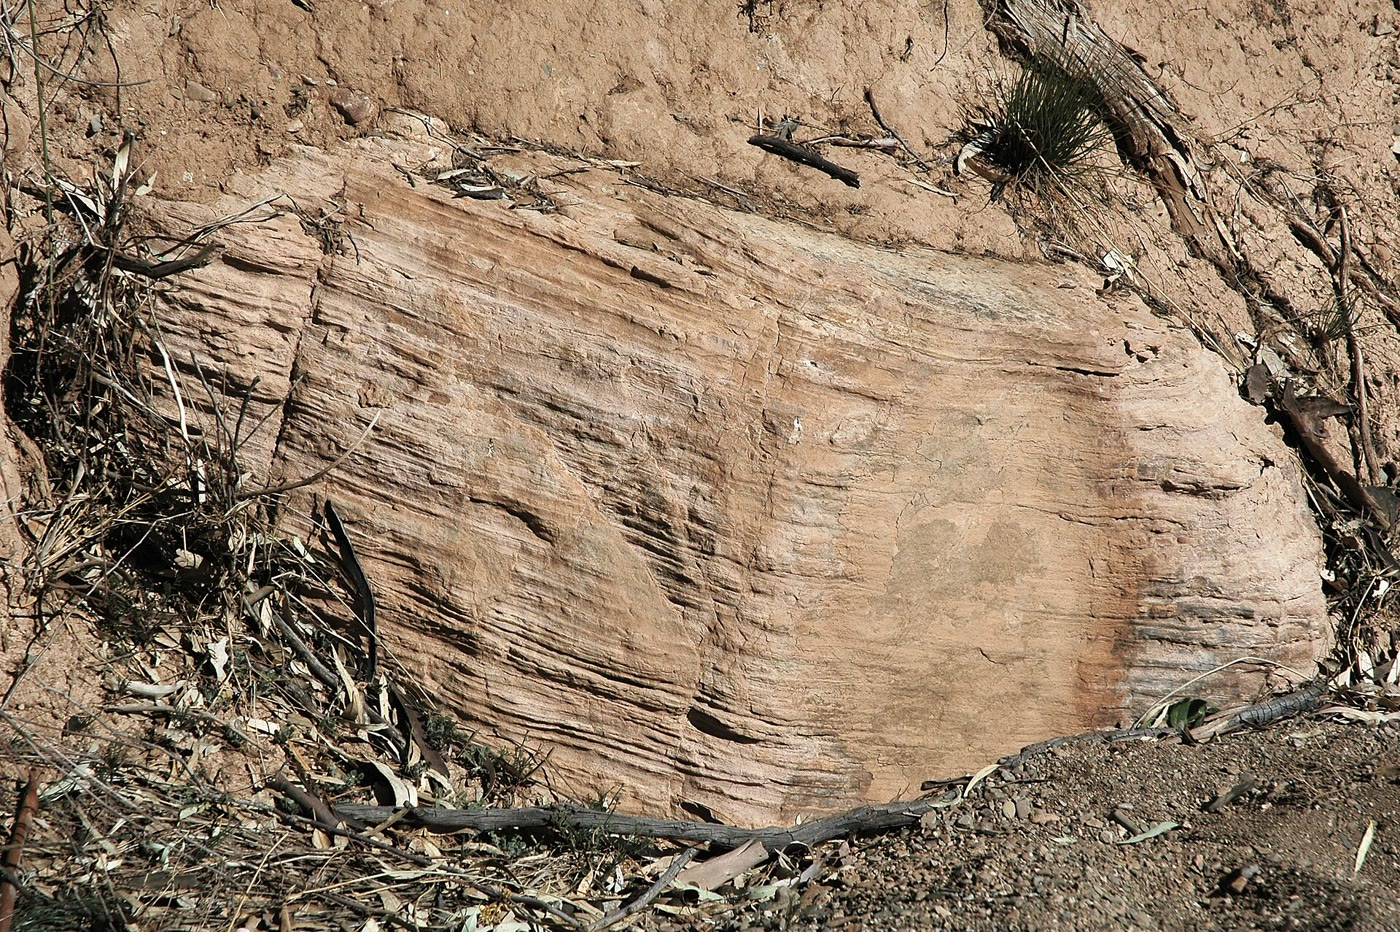
\includegraphics[width=0.66\linewidth]{images/book4/b2-18-cap-carbonate.jpg}
\par\smallskip{\small Een \omterm{def:b2:precambrian-earth:snowball}{kapcarbonaat}: gelamineerde dolosteen van de Nuccaleena-formatie,
Flinders Ranges, Zuid-Australië, rustend op de afzettingen van de Marinoische ijstijd
(de lagen zijn gekanteld). Foto James St.~John, CC~BY~2.0 (Wikimedia Commons).}
\end{omfigure}

Twee sneeuwballen van het Cryogenium zijn nu gedateerd met uranium--loodouderdommen op zirkonen uit vulkanische
as en met renium--osmiumouderdommen op schalies rijk aan organisch materiaal. De Sturtische ijstijd begon tussen 717.5 en
\qty{716.3}{Ma} en eindigde tussen 659.3 en \qty{658.5}{Ma}: \qty{58}{Myr} ijs, met
begin en einde overal ter wereld gelijktijdig. De Marinoische ijstijd begon tussen 649.9 en
\qty{639.0}{Ma}, ruw gedateerd, en eindigde tussen 636.0 en \qty{634.7}{Ma}: minstens
\qty{3}{Myr}. Elk eindigt met één enkel \omterm{def:b2:precambrian-earth:snowball}{kapcarbonaat}, nooit met meerdere. IJzerformaties,
een miljard jaar afwezig, keren terug in de glaciale afzettingen van de Sturtische ijstijd. Minstens één eerdere
sneeuwbal, in het Siderium rond \qty{2.4}{Ga}, viel samen met de GOE; tussen de twee
episoden, gedurende zo'n \qty{1.5}{Gyr}, zijn bijna geen ijskappen bekend.
% ledger: hoffman17:ages, hoffman17:cryochrons, hoffman17:cap, hoffman17:models, hoffman17:earlier

\begin{history}[Van een vreemde hypothese tot een gedateerde theorie]
In 1964 vestigde W.~B. Harland de aandacht op het bewijs voor een laat-precambrische ijstijd. In
1968 en 1969 vonden M.~I. Budyko, en W.~D. Sellers met een vergelijkbaar model, dat de
\omterm{def:b2:precambrian-earth:ice-albedo}{ijs--albedoterugkoppeling} het ijs tot aan de evenaar kon laten uitbreiden zodra het ver genoeg oprukte; een
wereldwijd bevroren Aarde leek toen een toestand zonder terugkeer, en dus een die nooit had plaatsgevonden.
In 1981 beschreven J.~Walker, P.~Hays en J.~Kasting de thermostaat van de silicaatverwering en
merkten op dat op een bevroren Aarde de koolstofdioxide van vulkanen zich zou ophopen tot het ijs
smolt: de toestand kon zichzelf beëindigen. In 1992 stelde J.~L. Kirschvink voor dat hij werkelijk had
plaatsgevonden, en noemde hem de ``Snowball Earth''; in 1998 publiceerden P.~F. Hoffman en collega's
``A Neoproterozoic Snowball Earth'', en de panglaciale tijdvakken gingen cryochronen heten. Geen
enkele cryogene glaciale afzetting was vóór 2004 radiometrisch gedateerd; de data hierboven zijn het
werk van de jaren sindsdien.
\end{history}
% ledger: hoffman17:history

Vulkanen zijn de uitweg. Op een Aarde die met ijs is bedekt, stoppen regen en rivieren bijna, en de
silicaatverwering met hen, en de koolstofdioxide die vulkanen afgeven, hoopt zich in de lucht op
tot het broeikaseffect ervan het ijs doet smelten.

\begin{proposition}[Opbouw van koolstofdioxide]\label{prop:b2:precambrian-earth:co2}
Als koolstofdioxide met een snelheid $F$ (massa per jaar) vrijkomt in een atmosfeer met massa
$M_{\text{a}}$ en gemiddelde molaire massa $\bar M$, zonder put, is de tijd die nodig is om de
volumemengverhouding ervan van bijna nul tot $x$ te brengen
\[
  \tau = \frac{x}{1 - x}\,\frac{M_{\mathrm{CO_2}}}{\bar M}\,\frac{M_{\text{a}}}{F} .
\]
\end{proposition}

\begin{proof}
De atmosfeer bevat $n = M_{\text{a}}/\bar M$ mol andere gassen. Het toevoegen van $n_c$ mol
koolstofdioxide maakt de mengverhouding ervan $x = n_c/(n + n_c)$, dus $n_c = n\,x/(1 - x)$, met massa
$n_c M_{\mathrm{CO_2}}$; met de snelheid $F$ duurt dit $\tau = n_c M_{\mathrm{CO_2}}/F$.
\end{proof}

\begin{example}[Hoe lang tot de ontsnapping?]\label{ex:b2:precambrian-earth:escape}
De hoogste voorkeursschatting van de huidige vulkanische uitstoot is \qty{0.26}{Gt}
koolstofdioxide per jaar. Schattingen van de
mengverhouding die nodig is om een cryogene sneeuwbal te beëindigen, lopen van 0.01 tot 0.1. Met $M_{\text{a}} =
\qty{5.1e18}{kg}$, $\bar M = \qty{28.97}{g.mol^{-1}}$ en $M_{\mathrm{CO_2}} =
\qty{44.01}{g.mol^{-1}}$ duurt $x = 0.01$ $\frac{0.01}{0.99}\times1.519\times\qty{5.1e18}{kg}
/ \qty{0.26e12}{kg.yr^{-1}} = \qty{0.30}{Myr}$, en $x = 0.1$ duurt \qty{3.3}{Myr}.
\end{example}
% ledger: usgs:volcanic-co2, hoffman17:co2, earth:Matm, earth:Mmol, ciaaw:abridged-2024
% values: co2_t001_Myr 0.301, co2_t01_Myr 3.311 (precambrian.py)

Een kolom zuivere koolstofdioxide die \qty{1}{bar} weegt boven de hele Aarde, zou met dezelfde snelheid
\qty{20}{Myr} duren, het getal dat Walker, Hays en Kasting gaven. Een paar miljoen jaar
is lang, maar de Sturtische ijstijd duurde \qty{58}{Myr}. Ofwel lag de drempel hoger, ofwel was de
ontgassing lager, ofwel had de bevroren Aarde nog putten: de verwering van de jonge zeebodem,
die onder ijs niet stopt, is één kandidaat. In het energiebalansmodel vraagt de ontsnapping dat
de effectieve emissiviteit van de sneeuwbal daalt tot zijn temperatuur \qty{263}{K} bereikt: onder
de cryogene Zon, \qty{94}{\percent} van de huidige, van 0.616 tot 0.472, een extra vasthouden van
zo'n \qty{39}{W.m^{-2}} (\cref{exo:b2:precambrian-earth:10}).
% ledger: hoffman17:co2, hoffman17:models, usgs:volcanic-co2
% values: one_bar_Myr 19.98, eps_melt_094 0.4716, forcing_melt_094 39.1 (precambrian.py)

Wanneer het ijs eindelijk aan de evenaar opengaat, werkt de terugkoppeling achteruit: donkere zee absorbeert meer
zonlicht, het ijs trekt terug, en in de modellen raast de ijsgrens in ongeveer
\qty{2}{kyr} naar de polen. De Aarde zit dan met een enorm broeikaseffect boven een donker oppervlak, een hete
nasleep. De verwering, zeer snel in dat klimaat, stort calcium, magnesium en bicarbonaat in
de zee, waar de kapcarbonaten neerslaan terwijl het smeltwater de plateaus overstroomt; het duurt
zo'n tien miljoen jaar om de koolstofdioxide weer omlaag te brengen. De ijskappen en de
kapcarbonaten, de ijzerformaties en de gelijktijdige ouderdommen zijn de reden waarom de meeste geologen nu aanvaarden
dat de cryogene sneeuwballen hebben plaatsgevonden, al wordt nog betwist hoe streng ze waren --- of een gordel van open
water aan de evenaar overleefde, zoals ``waterbelt''-modellen voorstellen.
% ledger: hoffman17:hysteresis, hoffman17:cap, hoffman17:debate

\section*{Oefeningen}\label{sec:b2:precambrian-earth:exercises}

Gegevens voor de oefeningen, tenzij anders vermeld: $\sigma = \qty{5.670e-8}{W.m^{-2}.K^{-4}}$;
$S_0 = \qty{1361}{W.m^{-2}}$; huidig albedo 0.294 en gemiddelde oppervlaktetemperatuur \qty{288}{K};
sneeuwbalalbedo 0.6; helling van \qty{263}{K} tot \qty{283}{K}; effectieve emissiviteit vandaag
0.616; wet van Gough $L/L_0 = 1/(1 + 0.4\,t/t_\odot)$ voor een tijd $t$ vóór heden, $t_\odot =
\qty{4.567}{Gyr}$; komatiietliquidus \qty{1616}{\celsius} bij \qty{32.2}{\percent} MgO,
helling \qty{18.0}{\celsius} per procent; halveringstijden \ce{^{238}U} \qty{4.468}{Gyr}, \ce{^{235}U}
\qty{0.704}{Gyr}, \ce{^{232}Th} \qty{14.0}{Gyr}, \ce{^{40}K} \qty{1.248}{Gyr}.
% ledger: const:sigma, earth:TSI, earth:albedo, earth:Tsurf, hoffman17:models, gough81:luminosity, connelly12:cai, so16:liquidus, iaea:isotopes

\begin{exercise}[$\star$]\label{exo:b2:precambrian-earth:1}
(a) Hoe lang duurden het \omterm{def:b2:precambrian-earth:eons}{Hadeïcum}, het \omterm{def:b2:precambrian-earth:eons}{Archaïcum} en het \omterm{def:b2:precambrian-earth:eons}{Proterozoïcum}? (b) Welk deel van de ouderdom
van de Aarde vormen ze samen? (c) Hoe oud was de Aarde toen de oudst bekende zirkoon
kristalliseerde, en toen de oudste gesteenten ontstonden?
\end{exercise}

\begin{exercise}[$\star$]\label{exo:b2:precambrian-earth:2}
Vandaag geeft de silicaataarde als geheel per kilogram \qty{1.917}{pW} af uit \ce{^{238}U},
\qty{0.082}{pW} uit \ce{^{235}U}, \qty{2.089}{pW} uit \ce{^{232}Th} en \qty{0.818}{pW} uit
\ce{^{40}K} ($\qty{1}{pW} = \qty{e-12}{W}$). (a) Bepaal elke bijdrage \qty{3}{Gyr} geleden, en
het totaal. (b) Met welke factor is de warmteproductie sindsdien gedaald? (c) Welke isotoop leidt
vandaag, en welke leidde toen?
\end{exercise}

\begin{exercise}[$\star$]\label{exo:b2:precambrian-earth:3}
Gebruik de komatiietthermometer. (a) Wat is de liquidus van een \omterm{def:b2:precambrian-earth:greenstone}{komatiiet} met
\qty{28}{\percent} MgO? (b) Welk MgO-gehalte komt overeen met \qty{1500}{\celsius}? (c) Een
stroom met spinifextextuur heeft een MgO-gehalte van het totale gesteente van \qty{38}{\percent}. Waarom mag zijn liquidus niet
van de lijn worden afgelezen?
\end{exercise}

\begin{exercise}[$\star$]\label{exo:b2:precambrian-earth:4}
Zet het volgende in volgorde en geef hun bij benadering ouderdom: de \omterm{def:b2:precambrian-earth:goe}{Grote Oxidatie}, de
eerste stromatolieten, het einde van de Marinoische ijstijd, de laatste gewone \omterm{def:b2:precambrian-earth:greenstone}{komatiieten}, de
oudste gesteenten, de tweede zuurstofstijging, de eerste fossielen van het Ediacarium, het einde van de
koepel-en-kielstructuren van de Pilbara.
\end{exercise}

\begin{exercise}[$\star\star$]\label{exo:b2:precambrian-earth:5}
(a) Ga na dat de effectieve emissiviteit van de huidige Aarde 0.616 is. (b) Bepaal het
sneeuwbalevenwicht onder de huidige Zon. (c) Toon aan dat het middelste evenwicht, \qty{275.5}{K}, voldoet aan
$R = E$ tot op \qty{0.5}{W.m^{-2}}. (d) Bepaal daar de hellingen van $R$ en $E$, en concludeer
dat het instabiel is.
\end{exercise}

\begin{exercise}[$\star\star$]\label{exo:b2:precambrian-earth:6}
(a) Bepaal met de wet van Gough het zonlicht \qty{2.4}{Ga} geleden en \qty{0.65}{Ga} geleden als fracties
van het huidige. (b) Is in het model op elke datum een warm klimaat mogelijk met de huidige emissiviteit?
(c) Hoffman en collega's schrijven dat de Zon van het Siderium ongeveer \qty{10}{\percent} zwakker was dan
de Zon van het Cryogenium. Ga dat na.
\end{exercise}

\begin{exercise}[$\star\star$]\label{exo:b2:precambrian-earth:7}
De Sturtische ijstijd duurde van \qty{716.9}{Ma} tot \qty{658.9}{Ma} (middens van de gedateerde intervallen),
de Marinoische van \qty{644.5}{Ma} tot \qty{635.4}{Ma}. (a) Bepaal hun duur en die van het
interglaciaal ertussen. (b) Welk deel van de periode Cryogenium, 720 tot \qty{635}{Ma},
bedekte ijs volgens deze getallen de Aarde? (c) Waarom is de duur van de Marinoische ijstijd slechts een
ruw getal?
\end{exercise}

\begin{exercise}[$\star\star$]\label{exo:b2:precambrian-earth:8}
(a) Hoe lang duurt het voordat vulkanen, met \qty{0.26}{Gt} per jaar en zonder put, de lucht op
een mengverhouding van koolstofdioxide van 0.05 brengen? (b) Hoeveel keer de \qty{278}{ppm} van 1750 is dat? (c) Als de helft van de uitstoot door de verwering van de
zeebodem werd opgenomen, hoe lang zou het dan duren?
\end{exercise}
% ledger: usgs:volcanic-co2, earth:Matm, earth:Mmol, ciaaw:abridged-2024, ipcc:erf-2xco2

\begin{exercise}[$\star\star$]\label{exo:b2:precambrian-earth:9}
Een neoproterozoïsche diamictiet bevat gekraste stenen, waarvan sommige in fijn gelamineerde modder liggen
die eronder omlaag is gebogen. (a) Wat vertelt die buiging? (b) Zijn paleobreedte is
\ang{10}. Waarom is dat van belang voor de sneeuwbalhypothese? (c) Hij wordt direct bedekt door een
roze gelamineerde dolosteen van enkele meters dik. Wat is dat, en wat legt hij vast?
\end{exercise}

\begin{exercise}[$\star\star\star$]\label{exo:b2:precambrian-earth:10}
Onder de cryogene Zon is $S = 0.94\,S_0$. (a) Toon aan dat in het model de warme toestand nog
bestaat, op het nippertje, maar dat er ook een sneeuwbal bestaat. (b) Bepaal de temperatuur van de sneeuwbal met
de huidige emissiviteit. (c) Bepaal de emissiviteit waarbij de sneeuwbal \qty{263}{K} bereikt en
ontdooit. (d) Zet de verandering van emissiviteit om in een extra vasthouden van langgolvige straling bij
\qty{263}{K}, in \unit{W.m^{-2}}.
\end{exercise}

\begin{exercise}[$\star\star\star$]\label{exo:b2:precambrian-earth:11}
(a) Toon met de kantelpunten van \cref{prop:b2:precambrian-earth:tipping} aan dat de breedte
van de hystereselus, $S_{\text{m}}/S_{\text{f}}$, niet van de emissiviteit afhangt, en
bereken ze. (b) Wat zou de lus smaller maken? (c) Waarom kan een sneeuwbal alleen ontdooien ver van
de omstandigheden waarin hij bevroor?
\end{exercise}

\begin{exercise}[$\star\star\star$]\label{exo:b2:precambrian-earth:12}
Leid de tijdconstante van het energiebalansmodel af in de buurt van het warme evenwicht, $\tau =
C/(E'(T^*) - R'(T^*))$, en bereken ze voor een gemengde oceaanlaag van \qty{50}{m} diep, met dichtheid
\qty{1025}{kg.m^{-3}} en soortelijke warmte \qty{3992}{J.kg^{-1}.K^{-1}}. Wat gebeurt er met $\tau$ wanneer het
zonlicht het linkerkantelpunt nadert, in dit model en in een model waarvan het albedo
geleidelijk met de temperatuur varieert?
\end{exercise}
% ledger: noaa:seawater-1025, teos10:cp0

\begin{problem}[{Weekendprobleem --- Een hetere jonge Aarde}]\label{pb:b2:precambrian-earth:1}
Dit probleem volgt de jonge Aarde van haar binnenste tot haar lucht. Gebruik de gegevens van de
oefeningen; de silicaataarde als geheel bevat in massa \qty{0.0203}{ppm} uranium, \qty{0.0795}{ppm}
thorium en \qty{240}{ppm} kalium, en haar isotopen geven \qty{95.13}{\micro W}
(\ce{^{238}U}), \qty{568.47}{\micro W} (\ce{^{235}U}), \qty{26.28}{\micro W} (\ce{^{232}Th}) en
\qty{28.47}{\micro W} (\ce{^{40}K}) af per kilogram isotoop. In massa bestaat uranium voor
\qty{99.29}{\percent} uit \ce{^{238}U} en voor \qty{0.711}{\percent} uit \ce{^{235}U}, en kalium voor
\qty{0.0120}{\percent} uit \ce{^{40}K}. Rond af op drie beduidende cijfers.

\noindent\textbf{Deel I --- Warmte van binnenuit.}
\begin{enumerate}
  \item Bepaal de warmte die elke isotoop vandaag afgeeft per kilogram silicaataarde, in
        \unit{pW.kg^{-1}}.
  \item Bepaal het totaal.
  \item Bepaal de vervalconstante van elke isotoop, in \unit{Gyr^{-1}}.
  \item Bepaal elke bijdrage \qty{2.7}{Gyr} geleden, toen de \omterm{def:b2:precambrian-earth:greenstone}{komatiieten} van Pyke Hill werden uitgestoten.
  \item Bepaal het totaal op dat moment, en de verhouding tot het huidige.
  \item Welke isotoop gaf toen de meeste warmte? Waarom geeft hij er vandaag zo weinig?
\end{enumerate}

\noindent\textbf{Deel II --- De Zon van het Archaïcum.}
\begin{enumerate}[resume]
  \item Bepaal met de wet van Gough het zonlicht \qty{2.7}{Ga} geleden als fractie van het huidige, en in
        \unit{W.m^{-2}}.
  \item Bepaal het warme evenwicht bij dat zonlicht met de huidige emissiviteit. Is het een geldige warme
        toestand van het model?
  \item Bepaal het sneeuwbalevenwicht bij dat zonlicht.
  \item Welke effectieve emissiviteit zou de Aarde op \qty{288}{K} houden met het warme albedo?
  \item Koolstofdioxide alleen had het kunnen doen met 0.004 tot \qty{0.03}{bar} bij \qty{2.5}{Ga}.
        Hoeveel keer de \qty{278}{ppm} van 1750 is dat, in een atmosfeer van ongeveer
        \qty{1}{bar}?
  \item Noem het proces dat de koolstofdioxide honderden miljoenen
        jaren op zo'n niveau hield.
\end{enumerate}

\noindent\textbf{Deel III --- Een sneeuwbal en zijn einde.}
\begin{enumerate}[resume]
  \item De eerste sneeuwbal, \qty{2.4}{Ga} geleden: bepaal het zonlicht toen als fractie van het huidige.
        Is de warme toestand van het model nog mogelijk met de huidige emissiviteit?
  \item Hoe lang duurt het met \qty{0.26}{Gt} koolstofdioxide per jaar om een
        mengverhouding van 0.1 te bereiken?
  \item Als de drempel onder de zwakkere Zon van het Siderium twee keer zo hoog was, 0.2, hoe lang dan?
  \item Welk gesteente legt het einde van een sneeuwbal vast, en hoe?
  \item Waarom hebben de ijzerformaties van de Sturtische ijstijd een oceaan zonder zuurstof onder het ijs nodig?
\end{enumerate}

\noindent\textbf{Deel IV --- De komatiietthermometer.}
\begin{enumerate}[resume]
  \item Ga de helling van de komatiietlijn na uit de twee experimenten.
  \item Een komatiietvloeistof van Pyke Hill had \qty{30}{\percent} MgO. Bepaal haar liquidus.
  \item Bepaal de liquidus van de \omterm{def:b2:precambrian-earth:greenstone}{komatiiet} van Barberton, \qty{32.2}{\percent} MgO.
  \item Bepaal de liquidus van een primair rugbasalt met \qty{12}{\percent} MgO.
  \item Hoe heet zou het basalt zijn met in plaats daarvan de helling van de Kilauea, \qty{20}{\celsius} per procent,
        uitgaande van het punt van Barberton? Hoeveel maakt de keuze van de helling uit?
  \item Waarom is het temperatuurverschil tussen de twee lava's groter dan het verschil in
        potentiële temperatuur tussen de archaïsche en de huidige mantel?
  \item Samengevat: hoeveel heter was de heetste archaïsche komatiietlava dan een primair basalt
        van de huidige ruggen?
\end{enumerate}
\end{problem}
% ledger: ms95:pm-trace, dye:isotope-heat, iaea:isotopes, gough81:luminosity, cz20:archean-air, ipcc:erf-2xco2, usgs:volcanic-co2, hoffman17:co2, so16:liquidus, helz98:glass-thermometer, pierru22:komatiite
